\chapter{Related Works}
\label{chap:related}

There has been several serious game for hemiplegic rehabilitation developed in the last few years. Similar to Hammer and Planks, these games also has some visualization feature which shows how the player performed so that the therapist is able to make the correct diagnosis. Thus, in this chapter, I first review some of these visualization. Then, since the nature of the input data is time series and movement data, I present some work in visualization which are related to this type of data.

\section{Visualization of Serious Game Result} 

Game result visualization is an integral part of a serious game used for rehabilitation since it's the feature which influence the accuracy of therapist analysis. Most serious game have an analytic feature, however the type of analysis presented depends on the nature of the game and the framework used in the rehabilitation. Therefore, for the purpose of this thesis, I only focus on reviewing serious game which are directed to hemiplegic patients rehabilitation.

In his paper, \cite{rahman} presents a rehabilitation framework for hemiplegic patients which combines the use of Kinect and LEAP\footnote{\url{https://www.leapmotion.com/product/desktop}} hand-tracking devices. These devices are attached to a 3D based game environment which was set to accommodate a set of primitive therapy motion such as forearm pronation/supination, shoulder and hip joint adduction/abduction, etc. Similar to Hammer and Planks, one of the game used in the framework requires user to navigate a plane by moving the hand to the right and left (hand-elbow flexion-extension). The recorded movement is then presented in line chart depicting the range of axis of elbow joint (180 degrees when fully extended and 20 degrees when fully flexed) over number of frames captured. Similarly, current visualization in Hammer and Planks also uses line chart to show average body movement over time. At first, line chart is used to represent Hammer and Planks gameplay, however in the end this approach is abandon since it's not intuitive enough. Details of this attempt can be found in chapter 4.

\begin{figure}
\centering
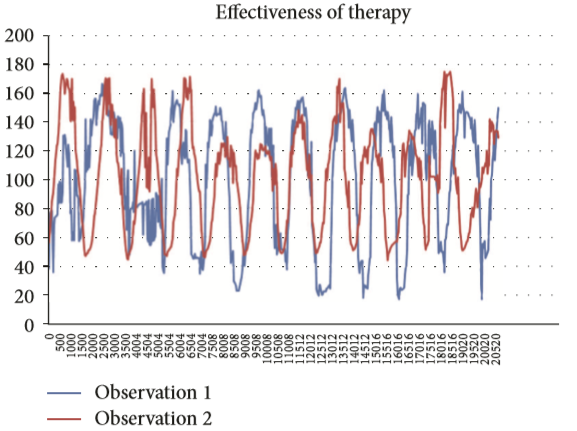
\includegraphics[width=110mm]{rahman_viz.png}
\caption{Visualization used in \cite{rahman} depicting the degree of forearm movement overtime}
\end{figure}

In \cite{green}, a virtual reality rehabilitation system for children with hemiplegia was developed using TUI\footnote{\url{https://en.wikipedia.org/wiki/Tangible_user_interface}}. The game itself is displayed on LCD and the player interact with the game by placing the TUI on top of moving targets shown on the LCD. In this system, performances are measured by speed, accuracy and trajectory(mean movement efficiency). However, unlike \cite{rahman}, this system doesn't provide an interface in which therapist can analyse the gameplay.

Similar to Hammer and Planks, \cite{rahman2} introduced a framework which uses Kinect attached to Second Life\footnote{\url{http://secondlife.com/}} serious game environment. The mission of the game is to follow a set of movement that have been configured beforehand by the therapist. During the game, the movement of each body joint  is recorded and saved in Session Recorder. Afterwards, a Kinematic Analytic component will process this data and visualize the quality of improvement metrics of each body joint movement. Each metric is visualized with a dotted line chart overtime as shown below.

\begin{figure}
\centering
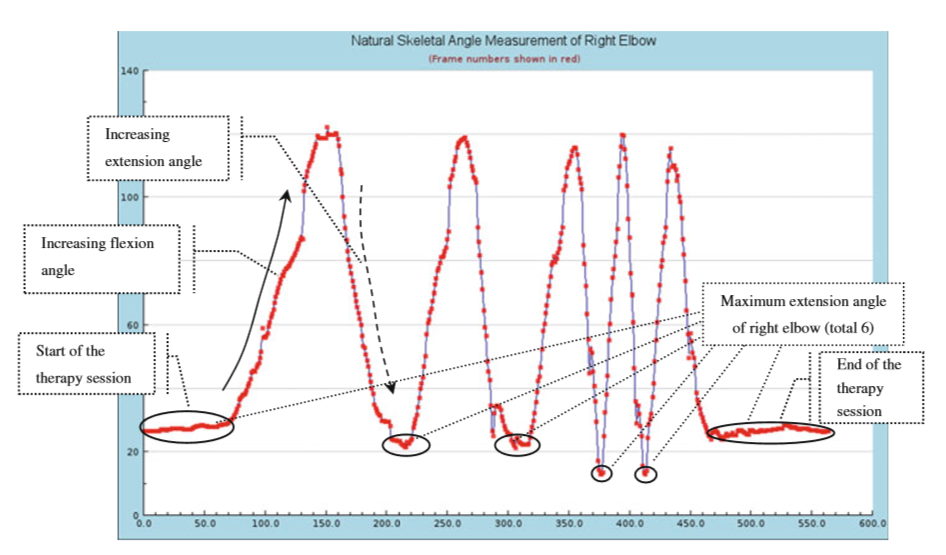
\includegraphics[width=110mm]{rahman2_elbowangle.png}
\caption{Visualization used in \cite{rahman2} depicting the speed of movement (m/s) of forearm overtime}
\end{figure}

discuss how the result of serious game are usually presented (couldn't find any specific paper discussing about this, but there are some paper about serious game which has some visualization to analyze the result of the game)
Discuss about state of the art game visualization

\section{Visualization of Time Series Data}
discuss visualization paradigm usually use to visualize time series data
\section{Visualization of Movement Data}
discuss paper about movement data visualization, ex: MotionExplorer, Andrienko's paper and book
\section{Stream Graph}
discuss examples of stream graph implementation, how it is used and for which kind of data

\section{Data Visualization Tool}
\subsection{D3.js}
general explanation of d3js and some example of how it is used to visualize time series and movement data.

\subsection{Three.js}
general explanation of three.js and some example.

